\documentclass[fleqn]{jbook}
\usepackage{physpub}
\usepackage{delarray}
\usepackage{txfonts}

\begin{document}

\def\therefore{.\raise1ex\hbox{.}.}
\renewcommand{\figurename}{fig.}


\begin{question}{問題3}{高瀬}

真空中に無限に長い直線状導線と半径$R$[m]の無限に長い中空の円筒導体が図1のように置かれている。導線は円筒の中心Oから$x$軸方向に$x_0$[m]($0 \le x_0 < R$)の位置にあるものとする。任意の点A(中心Oから距離r[m]、x軸からの角度$\phi$[rad])での動径方向と円周方向の電場を$E_r,E_\phi$[V/m]、磁束密度を$B_r,B_\phi$[Wb/m$^2$]として、以下の設問に答えよ。ただし、真空中の誘電率と透磁率を$\epsilon_0,\mu_0$とし、SI単位系(MKSA単位系)を用いるものとする。
\\

まず、導線が円筒の中心Oにある場合($x_0=0$)を考える。以下の設問に答えよ。
\\

\begin{enumerate}
	\item 導線に電流$I$[A]が紙面の下から上の方向に、円筒導体にはその反対方向に電流$I$[A]が一様に流れているとする。円筒内($r<R$)及び円筒外($r>R$)の各領域で、磁束密度$B_r,B_\phi$[Wb/m$^2$]を求めよ。
	\\
	\item 導線が$\lambda$[C/m]の線電荷密度(単位長さ当りの電荷)で一様に帯電している場合を考える。ただし、円筒は接地されているものとする。
	\\
	\\
	(a)円筒内($r<R$)及び円筒外($r>R$)の各領域で、電場$E_r,E_\phi$[V/m]を求めよ。
	\\
	\\
	(b)円筒面に生じる面電荷密度$\sigma$[C/m$^2$]と単位長さ当りの総電荷量$\lambda_t$[C/m]を求めよ。
	\\
	\\
	(c)円筒が接地されずに絶縁されていた場合、電場は円筒内と円筒外でどうなるか。ただし、絶縁前に帯電はされていないものとする。
	\\
	\\
	\newpage
	 次に、導線が円筒導体の中心Oからずれている場合($0<x_0<R$)を考える。以下の問いに答えよ。
	\\
	\item 設問1と同様に、導線に電流$I$[A]が紙面の下から上の方向に、円筒導体にはその反対方向に電流$I$[A]が一様に流れている。円筒外($r>R$)での磁束密度$B_r,B_\phi$[Wb/m$^2$]を求めよ。
	\\
	\item 設問2と同様に、導線が$\lambda$[C/m]の線電荷密度(単位長さ当りの電荷)で一様に帯電している。ただし、円筒は接地されているものとする。
	\\
	\\
	(a) 円筒導体に対する電気映像が、中心Oから$x$軸方向に$R^2/x_0$離れた位置にある線電荷密度-$\lambda$の無限に長い導線であることを示し、円筒内での電場$E_r,E_\phi$[V/m]を求めよ。
	\\
	\\
	(b) 円筒面に生じる面電荷密度$\sigma$[C/m$^2$]を求めよ。
	\\
	\\
	(c) 円筒を左右半分に分けて考えた時、$x>0$の部分($0^{\circ} \le \phi < 90^{\circ}及び270^{\circ} < \phi \le 360^{\circ}$)と$x<0$の部分($90^{\circ} < \phi <270^{\circ}$)の半円筒面に帯電する単位長さ当りの電荷$\lambda_+,\lambda_-$[C/m]をそれぞれ求め、
	\begin{eqnarray}
	\frac{\lambda_+ - \lambda_-}{\lambda_+ + \lambda_-} = S \cdot x_0
	\end{eqnarray}
	となる$S$を求めよ。ただし、$x_0 \ll R$として考えよ。
\end{enumerate}

\begin{figure}[htbp]
	\begin{center}
%	\includegraphics[width = .6\linewidth]{2002phy3q.eps}  
	\includegraphics[width=.4\linewidth]{2002physQ3_1.eps}  
	\caption{}
	\end{center}
\end{figure}

\end{question}


\begin{answer}{問題3}{高瀬}
\begin{enumerate}
	\item 
	\begin{itemize}
	
	\item $r<R$のとき \\
	アンペールの法則より、
		\begin{eqnarray}
		2\pi r \cdot B_\phi = \mu_0 I から B_\phi = \frac{\mu_0 I}{2 \pi r} [Wb/m^2]\\
		 (向きは紙面の上から見て反時計回り) \\
		B_r = 0 [Wb/m^2]
		\end{eqnarray}
	
	\item $r>R$のとき \\
	導線を流れる電流と円筒を流れる電流の向きが逆なので、アンペールの法則より、
		\begin{eqnarray}
		B_r = 0  [Wb/m^2]\\
		B_\phi = 0[Wb/m^2]
		\end{eqnarray}
	
	\end{itemize}
	\item 
	(a) 
		\begin{itemize}
		\item $r<R$のとき \\
		ガウスの法則より
		\begin{eqnarray}
	  (2 \pi r) \Delta l E_r = \frac{\lambda \Delta l}{\epsilon_0} \\
		ゆえに 中心から外へ向かう向きにE_r = \frac{\lambda}{2 \pi \epsilon_0 r} [V/m]\\
		また、	E_\phi = 0 [V/m]
		\end{eqnarray}
		\item $r>R$のとき \\
		接地されているので円筒には$-\lambda$の電荷が誘起されるので円筒の外から
		見ると内部の総電荷は0になる。よってガウスの法則より、
		\begin{eqnarray}
			E_r = 0  [V/m]\\
			E_\phi = 0 [V/m] \\
		\end{eqnarray}
		\end{itemize}

	(b) \\
		接地されているの円筒には$-\lambda$の電荷が誘起される。よって、
		\begin{eqnarray}
			\lambda_t = -\lambda [C/m]
		\end{eqnarray}
		このとき円筒面内に生じる面電荷密度は$\sigma$は、
		\begin{eqnarray}
			\sigma = - \frac{\lambda}{2 \pi R} [C/m^2]
		\end{eqnarray}
		
	(c)  \\
		絶縁前に帯電していないので、円筒面上の全電荷は0となり、この円筒面から
		出る電束は0である。ゆえに、電場は円筒内と円筒外で等しくなり、
		$E_r = \frac{\lambda}{2\pi\epsilon r}[V/m],E_\phi=0[V/m]$となる。
		\\
	
	\item
	
    $r>R$においては、円筒上の電流が作る磁場は、原点に置いた無限に長い導線を流れる電流が作る磁場と等しい。そこで、原点に置かれた無限に長い導線を流れる電流(流れる向きは紙面の上から下)と$x_0$に置かれた無限に長い導線を流れる電流(流れる向きは紙面の下から上)の作る磁場の重ね合わせを考えればよい。ここで、原点からの距離$r_1$[m]、$x$軸からの角度$\phi_1$[rad]での磁場を$B_{r1}$[Wb/m$^2$]、$x_0$からの距離$r_2$[m]、$x$軸からの角度$\phi_2$[rad]での磁場を$B_{r2}$[Wb/m$^2$]とする。このとき、
    \begin{eqnarray}
    	B_{r1} = 0  \quad B_{\phi 1} = \frac{\mu I}{2 \pi r_1} \\
    	B_{r2} = 0  \quad B_{\phi 2} = \frac{\mu I}{2 \pi r_2} \\
    \end{eqnarray}
    重ね合わせて、
    \begin{eqnarray}
    	B_\phi  = -B_{\phi 1} + B_{\phi 2} \cos \alpha 
    			= - \frac{\mu I}{2 \pi} (\frac{1}{r_1} - \frac{\cos \alpha }{ r_2}) \\
    	B_r = -B_{\phi 2} \sin \alpha = -\frac{\mu I}{2 \pi r_2} \sin \alpha
    \end{eqnarray}
    
    ただし、
    \begin{eqnarray}
    	r_1 &=& r \\
    	r_2 &=& \sqrt{r_1^2 + x_0^2 -2 r_1 x_0 \cos \phi_1} \\
    		&=&\sqrt{r^2 + x_0^2 -2 r x_0 \cos \phi_1} \\
		\phi_1 &=& \phi \\
    	\alpha &=& \phi_1 - \phi_2 \qquad (\alpha < \frac{\pi}{2})
    \end{eqnarray}

また、
	\begin{eqnarray}
		\frac{x_0}{\sin \alpha} = \frac{r_2}{ \sin \phi_1} より、
		r_2 \sin \alpha = x_0 \sin \phi_1 \\
		\frac{\cos \alpha}{r_2} = \frac{\sqrt{1-\sin ^2 \alpha}}{r_2}
	\end{eqnarray}
	を用いて整理すると、
	\begin{eqnarray}
		B_r = \frac{\mu I x_0 \sin \phi}{2 \pi (r^2 + x_0^2 - 2 r x_0 \cos \phi)}  \quad [Wb/m^2]\\
		B_\phi = -\frac{\mu I }{2 \pi}(\frac{1}{r} - \frac{r-x_0 \cos \phi}{r^2+x_0^2-2 r x_0 \cos \phi}) \quad [Wb/m^2]
	\end{eqnarray}
	\\
	
	\item
	(fig.\iref{souji})のようにO,B,C,D,Eをとる(問題文の図にあるAと同一平面上であり、C,Bのx座標はそれぞれ$x_0,\frac{R^2}{x_0}$である。)。\\
	\begin{figure}[htbp]
 		\begin{center}
   		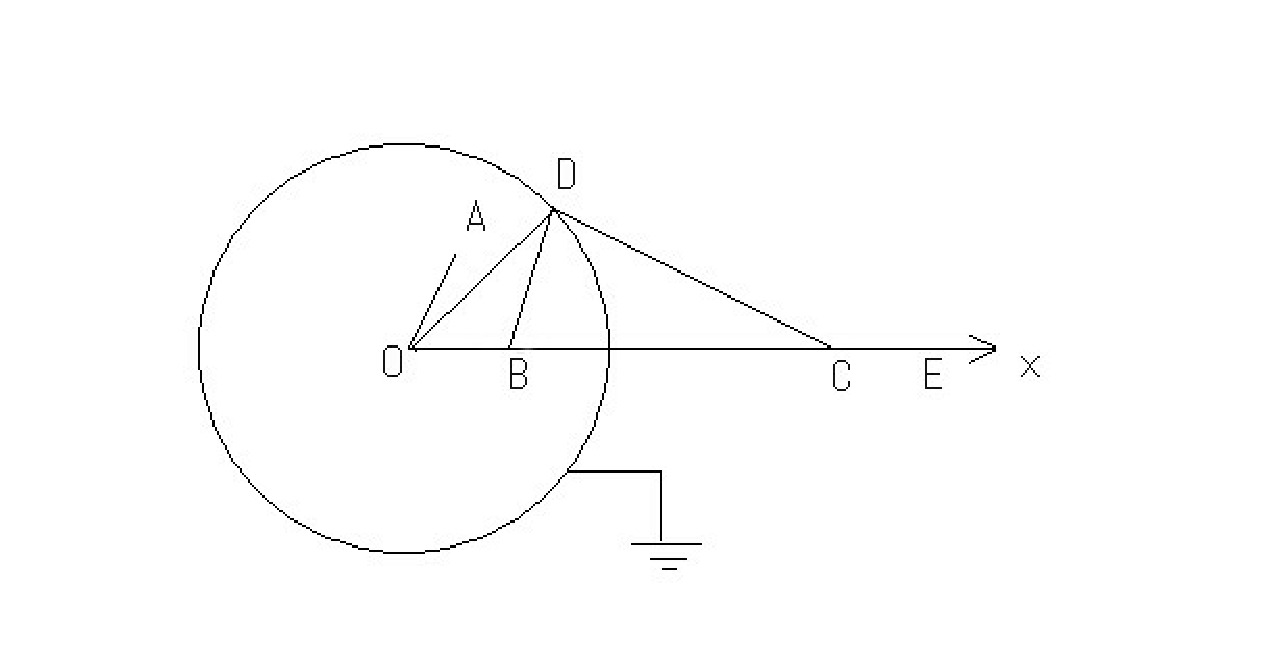
\includegraphics[width = .7\linewidth]{2002phy3a.eps}
   		\caption{} \ilabel{souji}
 		\end{center}
	\end{figure}
	\\
	このとき$\triangle ODB,\triangle OCD$は$x_0:R=R:\frac{R^2}{x_0}$より相似なので$DB=l_1$とすると、$CD=\frac{R}{x_0} l_1$となる。ここで$Bから\rho_2$かつ$Cから\rho_3$離れた点の電位は$\frac{\lambda}{2 \pi \epsilon_0} \ln \frac{\rho_2}{\rho_3} +(定数)$と表されるので、$\rho_2 = l_2, \rho_3 = \frac{R}{x_0} l_2$とすると、$\frac{\rho_2}{\rho_3} = \frac{x_0}{R} = (定数)$となるので、円筒面での電位が等電位となり接地された条件を満たすので、電気映像は$\frac{R^2}{x_0}$離れた$-\lambda$の無限に長い導線である。
	\\
	次に円筒内での磁場を求める。$\angle DCB=\phi_2$,$\angle DBE = \phi_3,DC=r_2,DB=r_3$とする。このときB,Cにおける導線上の電荷が作る電場$E_{r2},E_{r3},E_{\phi_2},E_{\phi_3}$は
  \begin{eqnarray}
		E_{r2} = \frac{\lambda}{2 \pi \epsilon_0 r_2} \quad E_{\phi2} = 0 \\
		E_{r3} = -\frac{\lambda}{2 \pi \epsilon_0 r_3} \quad E_{\phi3} = 0 \\
	\end{eqnarray}
	よって、A点での電場はこれらを重ね合わせて、
	\begin{eqnarray}
		E_r = E_{r2} \cos \theta_2 + E_{r3} \cos \theta_3
			= \frac{\lambda}{2 \pi \epsilon_0} 
			(\frac{\cos \theta_2}{r_2}-\frac{\cos \theta_3}{r_3}) \\
		E_\phi = E_{r2} \sin \theta_2 + E_{r3} \sin \theta_3
			= \frac{\lambda}{2 \pi \epsilon_0} 
			(\frac{\sin \theta_2}{r_2}-\frac{\sin \theta_3}{r_3}) \\
	\end{eqnarray}
	ただし、$i=2,3$について
	\begin{eqnarray}
		\theta_i \equiv \phi_i - \phi \\
		r_i^2 = r^2+x_i^2-2rx_i \cos \phi \qquad (x_2 = x_0, x_3 = \frac{R^2}{x_0})
	\end{eqnarray}
	また、$i=2,3$について
	\begin{eqnarray}
		正弦定理より、\frac{\sin \theta_i}{r_i} = \frac{x_i}{r_i^2}\sin \phi \\
		\frac{\cos \theta_i}{r_i} = \pm \frac{\sqrt{1-\sin^2 \theta_i}}{r_i}
		=\frac{r-x_0 \cos \phi}{r_i^2} \\  
	\end{eqnarray}		 
	となるので、

	\begin{eqnarray}
		E_\phi = \frac{\lambda}{2 \pi \epsilon_0}
		(\frac{x_0}{r^2+x_0^2-2rx_0 \cos \phi}
		-\frac{x_0R^2}{x_0^2r^2+R^4-2rx_0R^2\cos\phi}) \sin \phi \quad [V/m]
		\\
		E_r = \frac{\lambda}{2 \pi \epsilon_0}
		(\frac{r-x_0\cos\phi}{r^2+x_0^2-2rx_0 \cos \phi}
		-\frac{x_0^2r-xR^2\cos\phi}{x_0^2r^2+R^4-2rx_0R^2\cos\phi}) \quad [V/m]
	\end{eqnarray}
	\\
	
	(b) 
	円筒面に生じる面電荷密度は
	\begin{eqnarray}
		\sigma = -\epsilon_0 E_r | _{r=R}
			=\frac{\lambda}{2 \pi (R^2+x_0^2-2Rx_0 \cos \phi)}(R-\frac{x_0^2}{R}) \quad [C/m^2]
	\end{eqnarray}
	\\
	
	(c)
	$x_0 \ll R$より、
	\begin{eqnarray}
		\sigma = \frac{\lambda}{2 \pi R^2 (1+\frac{x_0^2}{R^2}-2\frac{x_0}{R}\cos \phi)}(R-\frac{x_0^2}{R})
		\simeq \frac{\lambda}{2\pi R^2}(R-\frac{x_0^2}{R})(1+2\frac{x_0}{R}\cos \phi)
		\end{eqnarray}
	よって、
	\begin{eqnarray}
		\lambda_+ &=& \int_0^{\frac{\pi}{2}}\sigma Rd\phi
					+\int_{\frac{3\pi}{2}}^{2\pi}\sigma Rd\phi \\
				&=&\frac{\lambda}{2\pi R}(R-\frac{x_0^2}{R})
				(\pi+4\frac{x_0}{R} ) \quad [C/m]\\
		\lambda_- &=& \int_{\frac{\pi}{2}}^{\frac{3\pi}{2}}\sigma Rd\phi \\
				&=&\frac{\lambda}{2\pi R}(R-\frac{x_0^2}{R})(\pi-4\frac{x_0}{R}) \quad [C/m]
	\end{eqnarray}
	これより、
	\begin{eqnarray}
		\frac{\lambda_+ - \lambda_-}{\lambda_+ + \lambda_- }
		= \frac{4 x_0}{\pi R}
	\end{eqnarray}
	となり、
	\begin{eqnarray}
		S=\frac{4}{\pi R} \quad [/m]
	\end{eqnarray}
	となる。
\end{enumerate}


\end{answer}


\end{document}
